\documentclass[a4paper]{article}

% --- Основные пакеты ---
\usepackage{graphicx}     % картинки
\usepackage{geometry}     % поля страницы
\usepackage{hyperref}     % гиперссылки
\usepackage{amsmath}      % математика
\ifPDFTeX
    \usepackage{amssymb}  % математические символы
\else
    \usepackage{unicode-math} % масштабируемые OpenType-матшрифты
\fi
\usepackage{float}        % [H] позиционирование фигур
\usepackage{iftex}        % определение движка (pdfLaTeX / XeLaTeX / LuaLaTeX)
\ifPDFTeX
    \usepackage[T2A]{fontenc} % кириллица
    \usepackage[utf8]{inputenc} % кодировка UTF-8
    \usepackage{anyfontsize}  % точные размеры шрифтов без подстановки
\else
    \usepackage{fontspec}     % системные шрифты с поддержкой кириллицы
    \setmainfont{Times New Roman}
    \setsansfont{Arial}
    \setmonofont{Consolas}
\fi
\usepackage[russian]{babel} % многоязычность
\usepackage{caption}      % настройка подписей
\usepackage[fontsize=13pt]{fontsize} % Размер шрифта

% --- Настройка страницы ---
\geometry{top=1.5cm, bottom=1.5cm, left=3cm, right=1.5cm}

% --- Настройка гиперссылок ---
\hypersetup{
    colorlinks,
    linkcolor=black,
    urlcolor=blue,
    citecolor=black
}

% --- Настройка подписей ---
\renewcommand{\figurename}{Рис.}
\captionsetup{labelsep=period}

% Заголовки разделов и подразделов без нумерации
\newcommand{\mainsection}[1]{%
    \phantomsection
    \section*{\centering\fontsize{16pt}{0pt}\selectfont\textbf{#1}}%
}
\newcommand{\subsectiontext}[1]{%
    \section*{\fontsize{13pt}{0pt}\selectfont\textbf{#1}}%
}

\begin{document}

% --- Титульная страница ---
\centering
Министерство науки и высшего образования Российской Федерации\\
Федеральное государственное автономное образовательное учреждение\\
высшего образования\\
«Южно-Уральский государственный университет\\
(национальный исследовательский университет)»\\
Институт естественных и точных наук

\setlength{\parskip}{7.5cm}

Отчет\\
Лабораторная работа №1.\\
Решение жестких систем ОДУ.

\setlength{\parskip}{5.9cm}

\raggedleft
\begin{minipage}{0.46\textwidth}
\raggedright
Выполнил: студент группы ЕТ-310\\
Тельнов С.М.\\
Проверил: преподаватель кафедры ВМ\\
Стариков Я.Е.
\end{minipage}

\setlength{\parskip}{5.9cm}

\centering
Челябинск — 2026

\setlength{\parskip}{0pt plus 1pt}
\newpage

% --- Содержание ---
\centering
\textbf{Краткое содержание}
\begin{itemize}
    \setlength{\parskip}{0.4cm}
    \item \hyperref[sec:theory]{\text{Теоретическая часть} \dotfill \pageref{sec:theory}}
    \item \hyperref[sec:practice]{\text{Практическая часть} \dotfill \pageref{sec:practice}}
    \item \hyperref[sec:conclusion]{\text{Вывод} \dotfill \pageref{sec:conclusion}}
\end{itemize}

\setlength{\parindent}{1.5em}

\raggedright

% --- Теоретическая часть ---
\label{sec:theory}
\mainsection{Теоретическая часть}

\subsectiontext{Жесткие системы ОДУ}

Рассмотрим задачу Коши для системы обыкновенных дифференциальных уравнений:
\begin{equation*}
    \bar{y}'(t) = \bar{f}(t, \bar{y}), \qquad \bar{y}(t_0) = \bar{y}_0,
\end{equation*}
где $\bar{y}(t) \in \mathbb{R}^n$ --- вектор неизвестных функций.

Система называется \textbf{жесткой} (stiff), если она устойчива по Ляпунову, но классические явные методы (Рунге---Кутты, Адамса) вынуждены выбирать шаг интегрирования значительно меньшим, чем того требует точность решения на рассматриваемом интервале. Жесткость характеризуется величиной разброса собственных значений матрицы Якоби $J = \partial \bar{f} / \partial \bar{y}$, вычисленной вблизи решения:
\begin{equation}
    \label{eq:stiffness}
    S = \frac{\max_i |\operatorname{Re} \lambda_i|}{\min_i |\operatorname{Re} \lambda_i|},
\end{equation}
где $\lambda_i$ --- собственные значения якобиана. Величина $S$ называется \textbf{числом жесткости} системы. Отрицательная вещественная часть собственных значений означает, что решения стремятся к устойчивому предельному режиму, при этом компоненты, соответствующие большим по модулю $\lambda_i$, затухают очень быстро, а компоненты с малыми $\lambda_i$ определяют поведение решения на большом интервале времени.

Для явных методов условие устойчивости имеет вид $|h \lambda_i| < C$, где $C$ --- константа метода (например, для классического метода Рунге---Кутты 4-го порядка $C \approx 2.78$). Если разброс собственных значений велик (отношение~\eqref{eq:stiffness} порядка $10^4$--$10^{17}$), явные методы вынуждены вести расчет с катастрофически малым шагом, определяемым самым быстрым компонентом, даже когда этот компонент уже практически затух и не влияет на решение. Именно поэтому для жестких систем применяют \textbf{неявные методы}, обладающие широкой областью устойчивости, вплоть до A-устойчивости (устойчивости во всей левой полуплоскости $\operatorname{Re} \lambda < 0$).

Ценой устойчивости становится необходимость на каждом шаге решать нелинейную систему уравнений (как правило, методом Ньютона), что требует вычисления матрицы Якоби и факторизации линейных систем. Однако шаг при этом ограничивается только требованиями точности, а не устойчивости, что делает неявные методы эффективными на жестких задачах.

\subsectiontext{Функция solve\_ivp}

\texttt{scipy.integrate.solve\_ivp} --- универсальный интегратор библиотеки SciPy для решения задачи Коши. Он поддерживает как явные, так и неявные методы, а его основные аргументы:
\begin{itemize}
    \item \texttt{fun} --- функция правой части системы, возвращающая $\bar{f}(t, \bar{y})$;
    \item \texttt{t\_span} --- интервал интегрирования $(t_0, T_k)$;
    \item \texttt{y0} --- вектор начальных условий;
    \item \texttt{method} --- схема интегрирования;
    \item \texttt{dense\_output=True} --- включение построения непрерывного интерполянта решения (\texttt{sol.sol(t)}), позволяющего вычислить решение в произвольной точке интервала.
\end{itemize}

По умолчанию интегратор самостоятельно контролирует локальную погрешность, адаптируя шаг (и порядок метода) в соответствии с заданными допусками \texttt{rtol} и \texttt{atol}. Внутри неявных методов на каждом шаге решается нелинейная система, поэтому дополнительно можно задать якобиан (\texttt{jac}); если он не указан, SciPy вычисляет его численно конечными разностями.

Доступные методы:
\begin{itemize}
    \item \texttt{'RK45'}, \texttt{'RK23'}, \texttt{'DOP853'} --- явные методы Рунге---Кутты разных порядков точности, не использующие якобиан; подходят для нежестких задач;
    \item \texttt{'Radau'} --- неявный метод Рунге---Кутты (коллокация на точках Радау IIA) 5-го порядка;
    \item \texttt{'BDF'} --- неявный многошаговый метод (формулы дифференцирования назад);
    \item \texttt{'LSODA'} --- адаптивный переключатель между явными (Адамса) и неявными (BDF) схемами.
\end{itemize}

\subsectiontext{Метод BDF}

\textbf{BDF} (Backward Differentiation Formulas, формулы дифференцирования назад) --- семейство неявных многошаговых методов, в которых производная в левой части аппроксимируется разностями \emph{по значениям решения в предыдущих узлах}. Для порядка $k$ схема имеет вид
\begin{equation*}
    \sum_{j=0}^{k} \alpha_j \bar{y}_{n+1-j} = h \, \bar{f}(t_{n+1}, \bar{y}_{n+1}).
\end{equation*}
Простейший вариант (BDF1, неявный метод Эйлера):
\begin{equation*}
    \bar{y}_{n+1} = \bar{y}_n + h \, \bar{f}(t_{n+1}, \bar{y}_{n+1}).
\end{equation*}
Свойства BDF:
\begin{itemize}
    \item устойчивы до порядка $k = 6$; методы BDF1 и BDF2 --- A-устойчивы, BDF3--BDF6 --- почти A-устойчивы ($A(\alpha)$-устойчивость), поэтому хорошо подходят для жестких задач;
    \item на каждом шаге требуется решение нелинейной системы, реализуемое методом Ньютона с численным или аналитическим якобианом;
    \item методы реализуют переменный шаг и переменный порядок: при гладком решении порядок повышается, при сложном поведении --- понижается;
    \item являются отраслевым стандартом (аналоги --- пакеты LSODE, VODE, CVODE из пакета SUNDIALS).
\end{itemize}
BDF эффективен для сильно жестких задач с большими интервалами интегрирования, когда быстрые компоненты решения затухают и дальнейшая динамика плавная.

\subsectiontext{Метод Radau}

\textbf{Radau} --- семейство неявных методов Рунге---Кутты (коллокационных методов) с этапами в точках Радау IIA. Метод 5-го порядка (три стадии) имеет вид
\begin{equation*}
    Y_i = \bar{y}_n + h \sum_{j=1}^{s} a_{ij} \bar{f}(t_n + c_j h, Y_j), \qquad
    \bar{y}_{n+1} = \bar{y}_n + h \sum_{j=1}^{s} b_j \bar{f}(t_n + c_j h, Y_j),
\end{equation*}
где $c_j$ --- коллокационные точки Радау. Свойства метода:
\begin{itemize}
    \item A-устойчивость и L-устойчивость: для компонентов с $|\lambda| \to \infty$ фактор затухания стремится к нулю, поэтому самые быстрые (жесткие) моды гасятся уже за один шаг без паразитных колебаний;
    \item высокий (5-й) порядок точности и надежная работа на резких переходных процессах и вблизи особенностей решения;
    \item на каждом шаге решается нелинейная система большой размерности, что дороже, чем у BDF, но метод устойчивее при сильных изменениях динамики.
\end{itemize}

Выбор метода в работе: для задач Робертсона и E5, где число жесткости достигает $10^{7}$ и $10^{17}$ соответственно, используется \texttt{BDF}; для умеренно жесткой биохимической модели, где решение претерпевает резкие переходные процессы, используется \texttt{Radau}.

\newpage

% --- Практическая часть ---
\label{sec:practice}
\mainsection{Практическая часть}

\subsectiontext{Задача 1. Система Робертсона}

Решим задачу химической кинетики, описываемую системой Робертсона, возникшей при описании химических реакций, протекающих в клетках некоторых растений. В системе три субстанции участвуют в трех химических реакциях:
\begin{equation*}
    A \to B, \qquad 2B \to C + B, \qquad B + C \to A + C.
\end{equation*}
Система ОДУ и начальные условия имеют вид
\begin{equation*}
    \begin{cases}
        y_1'(t) = -k_1 y_1(t) + k_3 y_2(t) y_3(t), \\
        y_2'(t) = k_1 y_1(t) - k_3 y_2(t) y_3(t) - k_2 y_2^2(t), \\
        y_3'(t) = k_2 y_2^2(t),
    \end{cases}
    \qquad y_1(0) = 1, \quad y_2(0) = 0, \quad y_3(0) = 0,
\end{equation*}
с параметрами $k_1 = 0.04$, $k_2 = 3 \cdot 10^7$, $k_3 = 10^4$. Здесь $\bar{y}(t)$ --- трехкомпонентный вектор неизвестных концентраций $y_i(t)$, $i = 1, 2, 3$, реагирующих веществ, $k_i$ --- константы скоростей химических реакций. Число жесткости системы имеет порядок $10^7$, поэтому использован метод \texttt{BDF}. Интервал интегрирования --- $(0, 10^{11})$.

\begin{figure}[H]
    \centering
    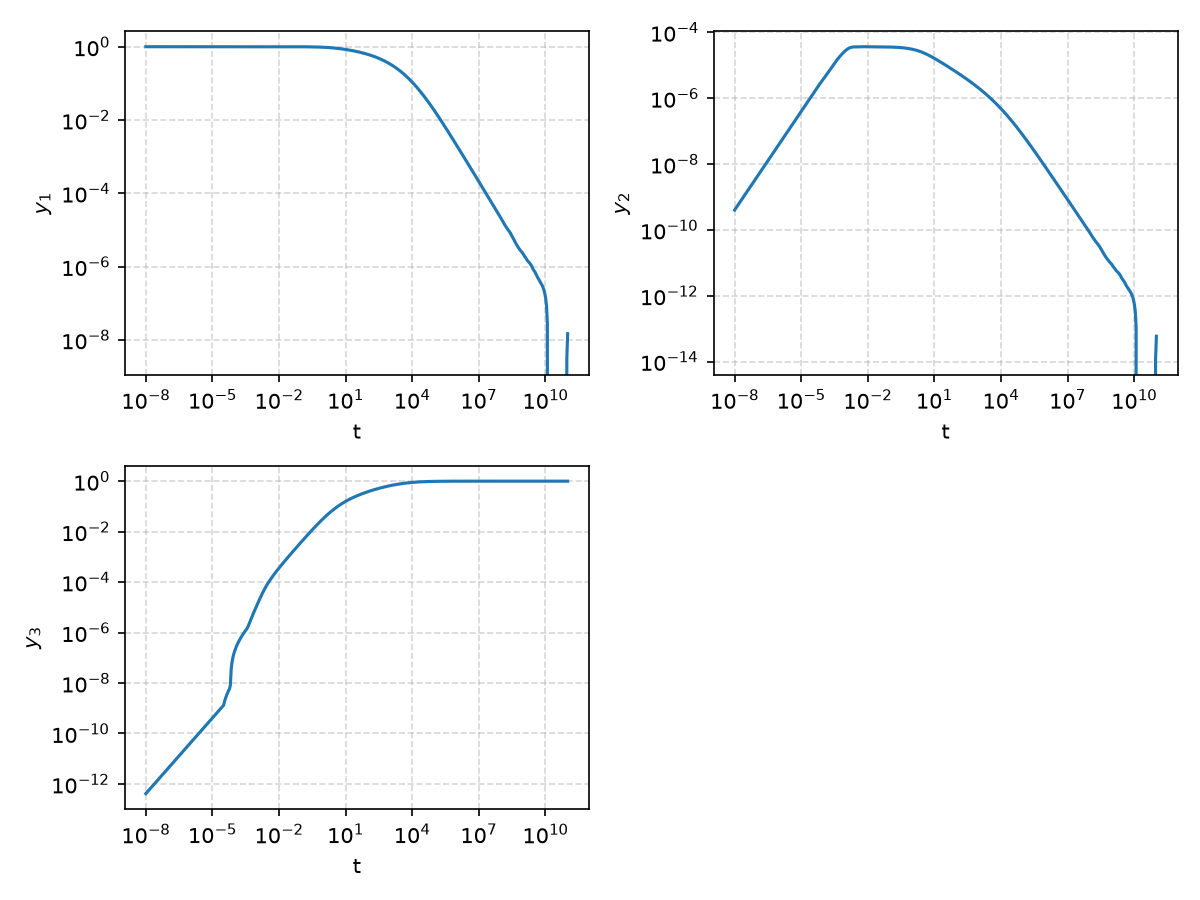
\includegraphics[width=0.9\textwidth]{../pictures/robertson.png}
    \caption{Решение системы Робертсона, полученное методом BDF}
    \label{fig:robertson}
\end{figure}

На рис.~\ref{fig:robertson} представлено решение системы, построенное по равномерной логарифмической сетке по времени на интервале $(0, 10^{11})$.

\subsectiontext{Задача 2. Задача E5 химической кинетики}

Решим задачу E5 химической кинетики, описываемую системой четырех химических реакций:
\begin{equation*}
    \begin{cases}
        y_1'(t) = -A y_1(t) - B y_1(t) y_3(t), \\
        y_2'(t) = A y_1(t) - M C y_2(t) y_3(t), \\
        y_3'(t) = A y_1(t) - B y_1(t) y_3(t) - M C y_2(t) y_3(t) + C y_4(t), \\
        y_4'(t) = B y_1(t) y_3(t) - C y_4(t),
    \end{cases}
\end{equation*}
с начальными условиями и параметрами
\begin{equation*}
    y_1(0) = 1.76 \cdot 10^{-3}, \qquad y_2(0) = y_3(0) = y_4(0) = 0,
\end{equation*}
\begin{equation*}
    A = 7.89 \cdot 10^{-10}, \qquad B = 1.1 \cdot 10^7, \qquad C = 1.13 \cdot 10^3, \qquad M = 10^6.
\end{equation*}
Время окончания расчета принято $T_k = 10^{13}$. Так как наибольшее отношение коэффициентов модели имеет порядок $10^{17}$, система считается жесткой, и для ее решения использован метод \texttt{BDF}.

\begin{figure}[H]
    \centering
    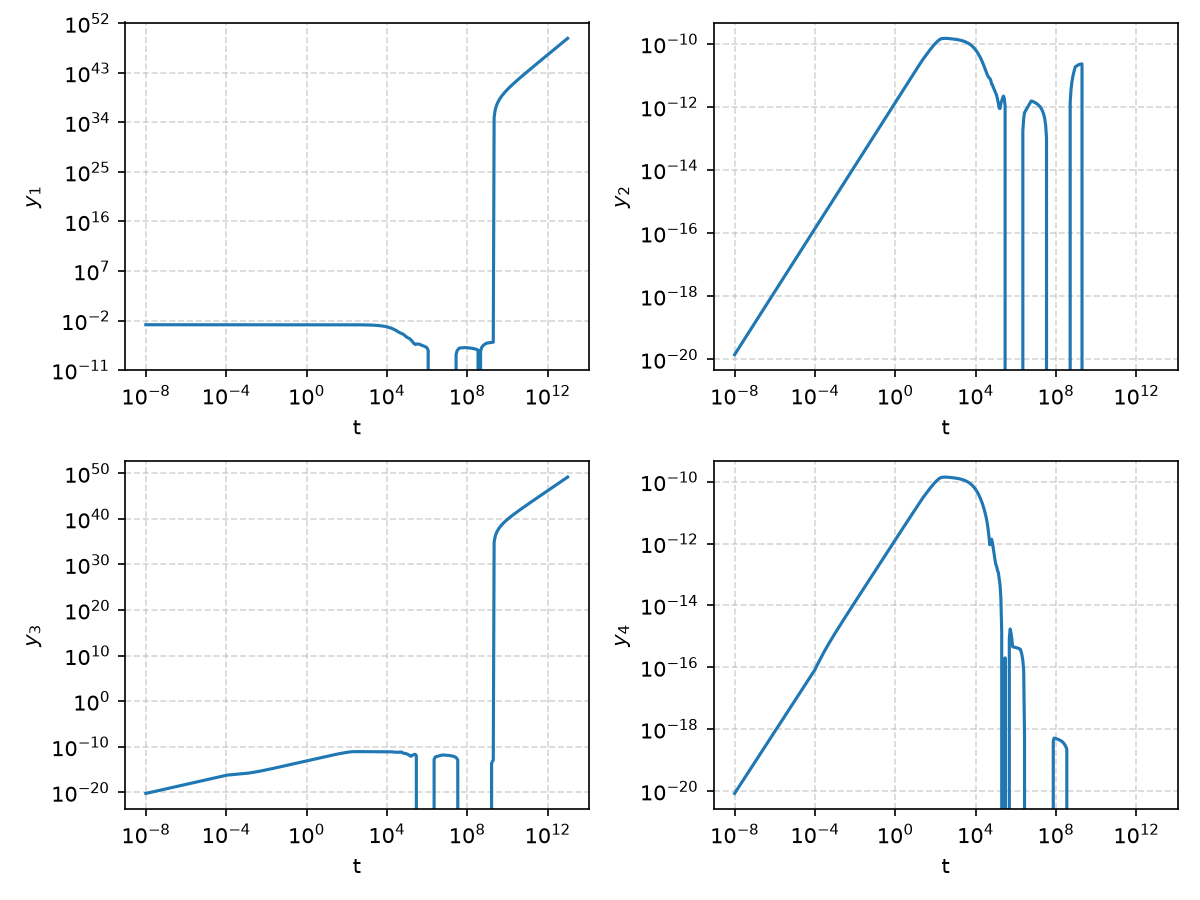
\includegraphics[width=0.9\textwidth]{../pictures/e5.png}
    \caption{Решение задачи E5, полученное методом BDF}
    \label{fig:e5}
\end{figure}

На рис.~\ref{fig:e5} представлено решение задачи E5 на интервале $(0, 10^{13})$, построенное аналогичным образом.

\subsectiontext{Задача 3. Биохимическая модель дифференциации растительной клетки}

Решим задачу, описывающую биохимическую модель дифференциации растительной клетки:
\begin{equation*}
    \begin{cases}
        y_1'(t) = -1.71 y_1(t) + 0.43 y_2(t) + 8.23 y_3(t) + 0.0007, \\
        y_2'(t) = 1.71 y_1(t) - 8.75 y_2(t), \\
        y_3'(t) = -10.03 y_3(t) + 0.43 y_4(t) + 0.035 y_5(t), \\
        y_4'(t) = 8.32 y_2(t) + 1.71 y_3(t) - 1.12 y_4(t), \\
        y_5'(t) = -1.745 y_5(t) + 0.43 y_6(t) + 0.43 y_7(t), \\
        y_6'(t) = -280 y_6(t) y_8(t) + 0.69 y_4(t) + 1.71 y_5(t) - 0.43 y_6(t) + 0.69 y_7(t), \\
        y_7'(t) = 280 y_6(t) y_8(t) - 1.87 y_7(t), \\
        y_8'(t) = -y_7'(t),
    \end{cases}
\end{equation*}
с начальными условиями
\begin{equation*}
    y_1(0) = 1, \quad y_2(0) = y_3(0) = y_4(0) = y_5(0) = y_6(0) = y_7(0) = 0, \quad y_8(0) = 0.0057.
\end{equation*}
Время окончания расчета принято $T_k = 421.8122$. Данная система считается умеренно жесткой. Решение получено методом \texttt{Radau}, который надежно обрабатывает как начальный переходный процесс, так и участки резкого изменения решения.

\begin{figure}[H]
    \centering
    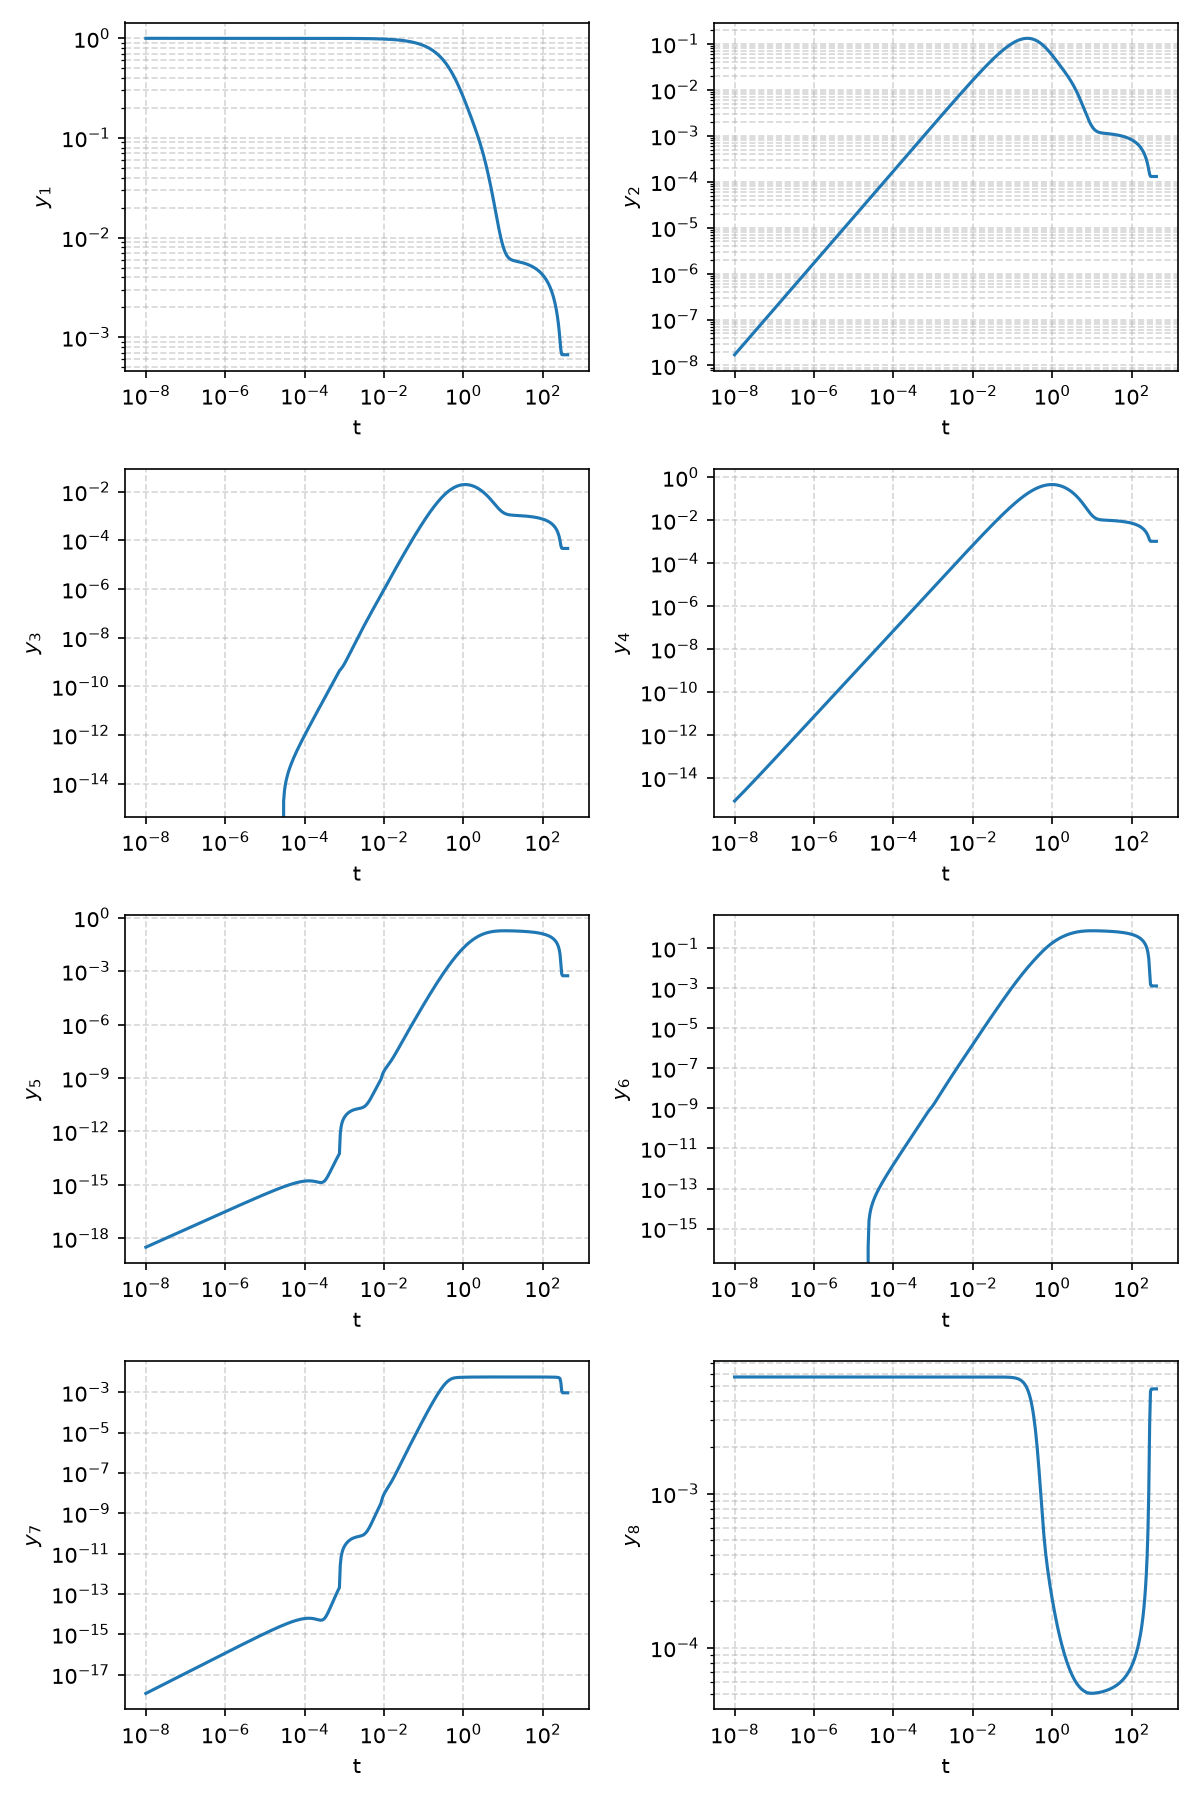
\includegraphics[width=0.9\textwidth]{../pictures/bio.png}
    \caption{Решение биохимической модели дифференциации растительной клетки, полученное методом Radau}
    \label{fig:bio}
\end{figure}

На рис.~\ref{fig:bio} представлено решение биохимической модели на интервале $(0, 421.8122)$.

\newpage

% --- Вывод ---
\label{sec:conclusion}
\mainsection{Вывод}

В ходе лабораторной работы изучены жесткие системы ОДУ и современные методы их численного решения. Реализовано численное решение трех классических жестких задач средствами библиотеки SciPy (функция \texttt{solve\_ivp}): системы Робертсона (метод \texttt{BDF}, интервал интегрирования до $10^{11}$), задачи E5 химической кинетики (метод \texttt{BDF}, интервал интегрирования до $10^{13}$) и биохимической модели дифференциации растительной клетки (метод \texttt{Radau}, интервал интегрирования до $421.8$). Решения построены графически на равномерных логарифмических сетках по времени.

Применение неявных A- и L-устойчивых методов \texttt{BDF} и \texttt{Radau} позволило устойчиво получить решения на столь широких интервалах времени: шаг интегрирования ограничивался лишь требованием точности, а не условием устойчивости. При использовании явных методов подобные задачи либо требуют катастрофически малого шага, либо приводят к численной неустойчивости.

\end{document}